\section{Simulation of heat conduction}
\label{sec_conduction}

Having briefly introduced transport {\tt Equation}s in {\psiboil} we move
forward to apply one of them to solve a simple steady heat conduction 
problem, governed by the equation:
%
\be
         \int_S \lambda \nabla T \, d{\bf S}
       = 0           
       \; \; \; \;
       [W]
  \label{eq_conduction}
\ee
%
It is clearly a special case of Eq.~\ref{eq_enthalpy}, without unsteady,
convective and source terms.

Let's consider a cubical computational domain, having dimensions 
$1 \times 1 \times 1$, and let's impose the following boundary conditions:
%
\begin{itemize}
  \item $T = 300 \; [K]$ at $x = 0$
  \item $T = 400 \; [K]$ at $x = 1$
  \item $\frac{\p T}{\p n} = 0$ everywhere else
\end{itemize}

The program which discretizes and solves this problem follows ({\tt 07-01-main.cpp}):
%
{\small \begin{verbatim}
      1 #include "Include/psi-boil.h"
      2
      3 const real L =  1.0;
      4 const int  N = 64;
      5
      6 /****************************************************************************/
      7 main(int argc, char * argv[]) {
      8
      9   boil::timer.start();
     10
     11   Grid1D g( Range<real>(0,L), N, Periodic::no());
     12   Domain d(g, g, g);
     13
     14   Scalar t(d), q(d);                          /* temperature and its source */
     15   Vector uvw(d);                              /* velocity field */
     16
     17   t.bc().add( BndCnd( Dir::imin(), BndType::dirichlet(), 300.0 ) ); /* b.c. */
     18   t.bc().add( BndCnd( Dir::imax(), BndType::dirichlet(), 400.0 ) ); /* b.c. */
     19   t.bc().add( BndCnd( Dir::jmin(), BndType::neumann() ) );          /* b.c. */
     20   t.bc().add( BndCnd( Dir::jmax(), BndType::neumann() ) );          /* b.c. */
     21   t.bc().add( BndCnd( Dir::kmin(), BndType::neumann() ) );          /* b.c. */
     22   t.bc().add( BndCnd( Dir::kmax(), BndType::neumann() ) );          /* b.c. */
     23
     24   Matter solid(d);                                  /* matter */
     25
     26   Krylov * solver = new CG(d, Prec::di());          /* linear solver */
     27
     28   Times time;                                       /* simulation time */
     29
     30   Enthalpy enth(t, q, uvw, time, solver, &solid);   /* enthalpy conservation
     31                                                        equation              */
     32   enth.diffusion_set(TimeScheme::backward_euler()); /* time stepping scheme */
     33
     34   AC multigrid( &enth );                            /* AMG solver for enth. */
     35
     36   t = 350.0;                                        /* initial "guess" */
     37
     38   multigrid.vcycle(ResRat(1e-4));                   /* solve linear system */
     39
     40   boil::plot = new PlotTEC();
     41   boil::plot->plot(t, "t");
     42
     43   boil::timer.stop();
     44   boil::timer.report();
     45 }
\end{verbatim}}
%
Although the problem being solved is simple, the program {\tt 07-01-main.cpp}
introduces many new concepts and each of them is presented in a separate subsection. 

\subsection{Boundary conditions}
\label{sub_sec_bc}

Boundary conditions are defined for fields, i.e.\ for {\tt Scalar}s and
for {\tt Vector}s. A class {\tt BndCnd}, defined in {\tt Src/Boundary}
holds the boundary conditions for various fields. {\tt BndCnd} can be 
defined in several ways (you can find them all in {\tt Src/Boundary/bndcnd.h},
but essentially, it is defined by {\em direction}, boundary condition {\em type} 
and {\em value}.

\subsubsection{Direction}

First parameter to define a boundary condition is {\em direction}. 
Direction can denote any of the logical six boundaries of computational 
{\tt Domain}, meaning: $i_{min}$ and $i_{max}$ (sometimes also referred 
to as {\em west} and {\em east}), $j_{min}$ and $j_{max}$ (or {\em south} 
and {\em north}), and $k_{min}$ and $k_{max}$ (or {\em bottom} and {\em top}). 
These directions are represented with ravioli object {\tt Dir}, which can 
assume one of the following values\footnote{Actually, {\tt Dir} is used as
if it was a constant defining direction. But a constant which is easy
to understand and for which compiler performs checking, when passed as
an argument}:
%
\begin{itemize}
  \item {\tt Dir::imin();} - west,
  \item {\tt Dir::imax();} - east,
  \item {\tt Dir::jmin();} - south,
  \item {\tt Dir::jmax();} - north,
  \item {\tt Dir::kmin();} - bottom and
  \item {\tt Dir::kmax();} - north boundary of the {\tt Domain}.
\end{itemize}
%
{\tt Dir} is a ravioli object and is defined in {\tt Src/Ravioli}.

\subsubsection{Boundary condition type}

Boundary condition type is stored in the ravioli class {\tt BndType} which,
since used only with {\tt BndCnd} is not defined in {\tt Src/Ravioli}
directory, but together with {\tt BndCnd}, in {\tt Src/Boundary}. 
{\tt BndType}, can assume one of the following values:
%
\begin{itemize}
  \item {\tt BndType::undefined();} 
  \item {\tt BndType::dirichlet();}
  \item {\tt BndType::neumann();}
  \item {\tt BndType::periodic();}
  \item {\tt BndType::inlet();}
  \item {\tt BndType::outlet();}
  \item {\tt BndType::wall();}
  \item {\tt BndType::symmetry();}
\end{itemize}
%
which are self-explanatory. ({\bf Check later if all {\tt BndType}s are 
applicable to all {\tt Equation}s})

\subsubsection{Boundary condition value}

This argument is optional. Namely, for some boundary conditions, such as 
symmetry and periodic, it does not have to be specified. If value is not
for other {\tt BndType}s, it is assumed to be equal to zero.
%
Value can be specified as a {\tt real} number, but also analytically,
as a function of $x$, $y$ and $z$ coordinates. That will be covered in
later sections. 

\subsubsection{Final form of boundary condition definition}

For example, to define a {\em Dirichlet} boundary condition at the 
{\em west} boundary of the {\tt Domain} (at $i = i_{min}$), with the
value of~300, we use the line:
%
{\small \begin{verbatim}
     BndCnd( Dir::imin(), BndType::dirichlet(), 300.0 );
\end{verbatim}}
%
To define a {\em Neumann} condition at the {\em north} boundary~($j = j_{max}$),
we do not have to specify the value, so the syntax is:
%
{\small \begin{verbatim}
     BndCnd( Dir::jmax(), BndType::neumann() );
\end{verbatim}}
%
These definitions are pointless if not assigned to fields representing
transported quantities. To achieve that, we use the member function: 
%
{\small \begin{verbatim}
     Scalar::bc().add( BndCnd & );
\end{verbatim}}
%
Program lines~17--22 assign various boundary conditions to {\tt Scalar t}.
The lines look cramped a bit, but that is because boundary condition 
object ({\tt BndCnd}) is defined at the place it is also passed as 
argument to {\tt Scalar::bc().add()}. To illustrate it further, program line~17,
with all the parts clearly denoted is shown below:
%
\bea
{\tt t.bc().add(} \; \overbrace{
              {\tt BndCnd(} 
                \overbrace{
                  \;
                  \underbrace{ {\tt Dir::imin()} }_{ \mbox{direction} }
                  , \;
                  \underbrace{ \; {\tt BndType::dirichlet()} }_{ \mbox{b.c.\ type} }
                  , \;
                  \underbrace{ \; {\tt 300.0} }_{ \mbox{value} }
                  \;
                }^{ \mbox{arguments to {\tt BndCnd(,,)}}} 
              )
            }^{ \mbox{{\tt BndCnd} is argument to {\tt add()}} } 
          \; 
{\tt );} \nonumber
\eea

\subsection{Matter}

There is a new
type of object defined in line~24, called {\tt Matter}. For every {\tt Equation}
solved by {\psiboil}, {\tt Matter} must be defined, bringing with it a suite of
physical properties featured in governing equations presented in Sec.~\ref{sec_equations}.
For this example, governed by the equation for steady conduction (Eq.~\ref{eq_conduction}
no property needs to be adjusted. Furthermore, {\tt Matter} can be defined as a
{\em mixture}, but that will not be covered in this section. Therefore, we simply
define an object of type {\tt Matter} now. 

\subsection{Krylov}

Next novelty is the object of type {\tt Krylov}, which is a linear solver
used to solve systems of discretized equations, created in line~26. Currently,
there are three solvers from Krylov sub-space family defined: Conjugate Gradient
(implemented as {\tt CG}), Bi-Conjugate Gradient~(as {\tt BiCG}) and Conjugate 
Gradient Squared~(implemented as class {\tt CGS}). 
{\tt Krylov} is a parent class to these three 
solvers and as such, it can {\em point} to each of them\footnote{Remember that
pointer to a parent class is also a pointer to all of it's children.}. A 
particular solver can be selected from one of the following constructors:

\begin{itemize}
  \item {\tt Krylov * solver = new CG  (d, Prec::di());} for CG   solver
  \item {\tt Krylov * solver = new BiCG(d, Prec::di());} for BiCG solver
  \item {\tt Krylov * solver = new CGS (d, Prec::di());} for CGS  solver
\end{itemize}

Constructor to each of the solvers takes a {\tt Domain} as first argument
and type of {\em preconditioner} as a second. Type of preconditioner is
defined by a ravioli object {\tt Preconditioner} and it can assume one of
the following values\footnote{This ravioli object is not defined in directory
{\tt Src/Ravioli}, because it is used only with {\tt Krylov} type solvers.}:
%
\begin{itemize}
  \item {\tt Preconditioner::di()} for diagonal,  
  \item {\tt Preconditioner::ic()} for Incomplete Cholesky, and  
  \item {\tt Preconditioner::no()} for no preconditioning.           
\end{itemize}

\subsection{Times}

Object of type {\tt Times} is defined in line~28. It defines the simulation
time, i.e.\ number of time steps which have to be performed, and a value
for the time step. In present case, which is steady\footnote{Steady cases are
an exception for kind of problems {\psiboil} aims at}, nothing needs to
be specified. 
{\tt Times} is a ravioli type object, defined in directory {\tt Src/Ravioli}. 
It is also useful in time-integration loops for unsteady problems, as will 
be shown below. 

\subsection{Transport equation}

Once we have field for transported quantity (here the temperature, {\tt Scalar t}), 
field for it's source (here {\tt Scalar q}), convective velocity field 
({\tt Vector uvw}), simulation time ({\tt Times time}) and a linear solver
({\tt Krylov * solver}), we can define a transport equation with the
constructor:
%
{\small \begin{verbatim}
     30   Enthalpy enth(t, q, uvw, time, solver, &solid); 
\end{verbatim}}
% 
Convective velocity field, source and time, {\em must} be provided, no matter
if problem involves transport by velocity, has any external sources, or is it
unsteady. It may look as an overhead, but keep in mind that {\em vast} majority 
of problems analyzed with {\psiboil} are {\em unsteady}, involve fluid flow 
and feature external {\em sources} on transported variables. Actually, it would
be an overhead to write additional constructors for these special cases which
occur very rarely. 
%
The form of constructor shown above is {\em the same} for all transport 
{\tt Equation}s implemented in {\psiboil}. Constructor for {\tt Equation},
such as the one in line~30, also discretizes the governing transport
equation, for this case, it is the enthalpy conservation defined 
with~Eq.~\ref{eq_enthalpy}.

\subsection{Time-stepping scheme}
\label{sub_sec_time_stepping}

For each transport equation, time stepping scheme can be set for {\em diffusive}
and {\em convective} terms. If nothing is specified, {\psiboil} uses  
default schemes, which are:
%
\begin{itemize}
  \item {\em Adams-Bashforth} for convection, and
  \item {\em Crank-Nicolson} for diffusive terms. 
\end{itemize}
%
For steady cases\footnote{Again: which is an exception}, time stepping 
scheme should be set to {\em steady}.
%
In this case, there is no convection, so setting the time-stepping scheme 
for convection is pointless. For diffusion, it is set with the line:
%
{\small \begin{verbatim}
     32   enth.diffusion_set(TimeScheme::steady()); 
\end{verbatim}}
% 
This setting uses {\tt Equation}'s member function {\tt diffusion\_set}
and ravioli object {\tt TimeScheme}, which can have one of the following
values:
%
\begin{itemize}
  \item {\tt TimeScheme::backward\_euler();} 
  \item {\tt TimeScheme::crank\_nicolson();}
  \item {\tt TimeScheme::adams\_bashforth();}
\end{itemize}
%

\subsection{Additive correction multigrid solver}

This case, since steady, results in relatively poorly conditioned linear
system of discretized equations. Therefore, it is sound to use a multigrid
procedure to accelerate it's convergence. {\psiboil} has only one multigrid
algorithm, based on Additive Correction (AC) scheme ({\bf add reference}). It
is defined in class~{\tt AC}. Algebraic multigrid is based on coarsening
discretized system of equations and solving these coarser (smaller) systems
faster, leading to faster reduction of residuals on finer (bigger) levels
as well. {\tt AC} is defined in line~34:
%
{\small \begin{verbatim}
     34   AC multigrid( &enth );  
\end{verbatim}}
% 
It takes the reference to {\tt Equation} as a parameter. Remember that
{\tt Equation} was already defined with a linear solver ({\tt solver}),
which will be used by {\tt AC} to {\em smooth} each refinement level. 

The solution of the liner system by {\tt AC} is invoked by:
%
{\small \begin{verbatim}
     38   multigrid.vcycle(ResRat(1e-4));
\end{verbatim}}
% 
which starts a "V" multigrid cycle and runs until residuals fall four
levels of magnitude. 

This program creates the following output:
%
{\small \begin{verbatim}
Domain level 4 created !
Domain level 3 created !
Domain level 2 created !
Domain level 1 created !
FILE: centered_coarsen.cpp, LINE: 6, coarsenig
Centered level 32 x 32 x 32 created !
Centered level 16 x 16 x 16 created !
Centered level 8 x 8 x 8 created !
Centered level 4 x 4 x 4 created !
Number of cycling levels: 5
FILE: centered_update_rhs.cpp, LINE: 14, conv_ts.N() = 0
Initial  res = 2.95794
Cycle 1; res = 0.062026
Cycle 2; res = 0.00803034
Cycle 3; res = 0.000562558
Cycle 4; res = 0.000247838
Converged after 4 cycles!
# Plotting: t_p000.dat
+==========================================
| Total execution time: 6.21 [s]
+------------------------------------------
| Time spent in enthalpy discretize: 0.03 [s]    (0.462963%)
| Time spent in vcycle             : 5.12 [s]    (79.0123%)
| Time spent in coarsening         : 0.04 [s]    (0.617284%)
| Time spent in plotting           : 1.21 [s]    (18.6728%)
| Time spent elsewhere: 0.08 [s]    (1.23457%)
+------------------------------------------
\end{verbatim}}
% 
The messages in the first five lines should be familiar. They are printed 
during the {\tt Domain} definition phase. Lines beginning with 
{\tt"Centered level ..."} are messages from the {\tt AC} multigrid solver, 
printed while it creates coarser levels. For this case, number of cycling levels,
including the finest one (defined by the user) is five. Lines beginning
with {\tt"Cycle ..."} print the residuals from each "V" cycle performed
in multigrid solver. It is generally an {\em excellent} sign if residuals 
fall by an order of magnitude in each cycle. More often they fall by 
a factor of five in each cycle. 
The output finishes with CPU-time statistics. In {\tt main.cpp} we
have defined only global timers
% \footnote{Sec.~\ref{sec_global}}
(lines~9, 43 and 44), but certain {\psiboil} subroutines have built-in 
local timers.
% \footnote{Sec.~\ref{sec_local}}. 
The output we got for this
program is typical. Very little time was spent in discretization of
governing equations (0.49~\%), approximatelly the same in {\tt Domain} 
coarsening (0.61~\%), but vaste majority of CPU time is spend in
V-cycle~(79~\%). For this simulation, particularly because it is
steady, a lot of time is spent in plotting as well~(18.7~\%). Only~(1.23~\%)
is spent in the parts of the code which are not measured, meaning that 
time monitors are properly placed. 

This data provides useful profiling information. It is
clear that any {\em tuning} of the code in the parts of the code which
discretize governing equations, will not bring the overall CPU-time down
considerably. 

\subsection{Final solution}

The final solution obtained by the program (stored in file: {\tt t\_p000.dat}
is given in Fig.~\ref{fig_temperature}. Clearly, the solution is linear,
ranging from~$T=300 \; [K]$ to $T=400 \; [K]$.

%---------------%
%               %
%  Temperature  %
%               %
%---------------%
\begin{figure}[ht]
  \centering
  \setlength{\unitlength}{1mm}
  \begin{picture}(100,85)(0,0)
    \thickbox{100}{85}
    \put(0,-3){\includegraphics[scale=0.45]{Figures/07-01-temp.eps}}
  \end{picture}
  \caption{Temperature field}
  \label{fig_temperature}
\end{figure}

\subsection{Exercise}

Note that {\tt AC} multigrid solver is optional. Try to modify the program
lines~34--38 to:
%
{\small \begin{verbatim}
     34// AC multigrid( &enth );                            /* AMG solver for enth. */
     35
     36   t = 350.0;                                        /* initial "guess" */
     37
     38   enth.solve(ResRat(0.001), "enthalpy");
\end{verbatim}}
%
With this modification, you do not create {\tt AC} multigrid solver (line~34 is a
comment) and you directly call Krylov solver to {\em solve} the discretized
equations for you. Compile and run this program. Visualize the results and compare
with the ones shown in~Fig.~\ref{fig_temperature}. What do you see? Can you 
comment on that? 

%---------------------------------------------------------------------nutshell-%
\vspace*{5mm} \fbox{ \begin{minipage}[c] {0.97\textwidth} %-----------nutshell-%
    {\sf Section \ref{sec_conduction} in a nutshell} \\  %-------------nutshell-%
   
      - To solve a transport equation in {\psiboil}, the following objects
      have to be used (in addition to {\tt boil::timer}, {\tt Grid1D} and
      {\tt Domain} introduced before): 
      \begin{itemize}
        \item {\tt Matter} - to define the physical properties of the
              matter (substance) under consideration,
        \item {\tt Krylov} - a member of the Krylov's subspace family of
              solvers for solving the discretized equations,
        \item {\tt Times} - object representing simulation time,
        \item Field variables represented by {\tt Scalar} and {\tt Vector} objects,
        \item {\tt BndType}, {\tt BndCnd} and {\tt Dir} to define boundary
              conditions, 
        \item Governing {\tt Equation} - such as enthalpy, species, momentum
              conservation,
        \item (optional) Setting the time stepping scheme with the {\tt TimeScheme} object.
        \item (optional) {\tt AC} multigrid solver.
      \end{itemize}

  \end{minipage} } %--------------------------------------------------nutshell-%
%---------------------------------------------------------------------nutshell-%
